\documentclass[11pt,a4paper]{article}
\usepackage{od}
\usepackage[utf8]{inputenc}
\usepackage[russian,main=ngerman]{babel}

\title{Über die Gesetze der Konstruktion technischer Systeme }

\author{B.I.Goldovsky}
\date{Februar 2018}

\begin{document}
\maketitle
\begin{quote}
  Original: \foreignlanguage{russian}{О законах построения технических
    систем}\footnote{\url{https://www.metodolog.ru/node/2164}.}.

  Erschienen in \foreignlanguage{russian}{ТРИЗ нужна России: проблемы
    технического творчества. Сб. ст.выпуск 2. – Чебоксары: Новое время, 2018.}
  S. 54 - 72.
  
  Übersetzt von Hans-Gert Gräbe, Leipzig, mit Unterstützung durch die freie
  Version von \texttt{deepl.com}.
\end{quote}

Die von G.S.Altshuller [1] vorgeschlagene Liste der Gesetze für die
Entwicklung technischer Systeme (TS) war wird ganz künstlich und bedingt in
die Gesetze„Statik“,„Kinematik“ und„Dynamik“ unterteilt. Schritt zu die
natürliche Klassifizierung dieser Gesetze wurde in den frühen 80er Jahren von
V.M.Petrov vorgenommen, der die Gesetze der„Statik“ werden die Gesetze der
Organisation genannt. (d.h. Konstruktion), sowie die Gesetze der„Kinematik“
und vereinigte„Dynamik“ zu„Evolutionsgesetzen“ (d.h. Entwicklung) [2], [3]
(offensichtlich unter Verwendung von mehr als seiner frühen Entwicklungen zu
diesem Thema). Fast zur gleichen Zeit auch der Autor dieses Artikels.  hat die
Entwicklung des Systems der Gesetzmäßigkeiten der Konstruktion und Entwicklung
technischer Systeme durchgeführt [4]. Zweck .  die Entwicklung war einfach:
das Thema zu verstehen. Infolgedessen gab es im Wesentlichen drei des
Augenblicks:
\begin{itemize}
\item das System der Muster ist tatsächlich viel komplexer als die Liste in
  [1];
\item Einige der Regelmäßigkeiten lassen sich deduktiv begründen;
\item vom System der Gesetzmäßigkeiten ist es notwendig, die Gesetze des
  TS-Aufbaus
\end{itemize}
zu trennen, und zwar Effizienz der TS, weil die Gesetze der Entwicklung
innerhalb der Gesetze der Konstruktion wirken.

Die letzte These, als methodologisch wichtig, wurde 1983 in den
Konferenzthesen [5] veröffentlicht.  (siehe auch [6]), wurde auch in späteren
Publikationen versucht, darauf aufmerksam zu machen. Aber .  ohne Erfolg. Es
ist durchaus verständlich, denn die Hauptwerke der TRIZ-Spezialisten nach den
Gesetzen Die Konstruktion und Entwicklung technischer Systeme hat sich
hauptsächlich auf die Beschreibung von Gesetzen konzentriert, ihre
Klassifizierung und Auswahl von Beispielen [7], [8]. Die Frage der Mechanismen
für die Funktionsweise der Gesetze, für die Diese methodologische These mag
wichtig gewesen sein, wurde aber nicht berücksichtigt.

\begin{emph}
  Ein solches Phänomen ist ganz typisch für die Entwicklung jeder
  wissenschaftlichen Erkenntnis. Wie in [9] erwähnt:„Die Wissenschaft bewegt
  sich wie mit dem Rücken zur Zukunft; sie drängt vorwärts und lässt uns
  überblicken der zurückgelegten Weg. Wer sich schneller bewegt und seine
  Zeitgenossen überholt, fällt aus dem Feld.  der Vision“.
\end{emph}

Im Jahr 2017 versuchte N.A.Shpakowski im Artikel [10] N.A.Schpakowski über das
Rechtssystem von V.M.Petrov den Prozess der Schaffung und TS-Entwicklung,
nannte die Gesetze der Organisation wesentlich und die Gesetze der Evolution
hilfreich. Dies ist die Einteilung ist nicht ganz korrekt, denn diese Gesetze
haben unterschiedliche Wirkungsbereiche. Doch gerade die Tatsache Die
Hervorhebung der besonderen Rolle der Gesetze der TS-Konstruktion ist
richtig. Was ist die Besonderheit der Gesetze?  des Gebäudes TS?

Es ist bekannt, dass alle TS Teil von zwei Beziehungssystemen sind: Natur und
Gesellschaft (menschliche Gesellschaft).  Sie werden von der Gesellschaft für
menschliche Bedürfnisse geschaffen, aber unter Verwendung des natürlichen
Substrats.  Was die technischen Widersprüche betrifft, so zeigte sich dies in
[11]: relations die Interdependenz der Konfliktparteien wird durch das
natürliche Substrat bestimmt (daher diese Beziehungen sind bedingungslos), und
die Beziehungen des Gegenteils werden durch Bewertungen der Gesellschaft
bestimmt (daher relativ, nicht bedingungslos). Ein ähnliches Bild ergibt sich
in Bezug auf die Gesetze von des Aufbaus und der Entwicklung der TS.

Es ist zu beachten, dass das Gesetz eine Zwangskategorie ist. Jedes
bedingungslose Gesetz sollte Folgendes bestrafen für die Nichteinhaltung
seiner Anweisungen. In dieser Hinsicht unterscheiden sich die Gesetze der
TS-Konstruktion erheblich von Entwicklungsgesetze (in ihrem Wesen und
Wirkungsmechanismus). Gesetze der TS-Konstruktion als Reflexion das natürliche
Substrat der Technologie ist bedingungslos: ihre Verletzung führt unmittelbar
zur Funktionsunfähigkeit des Fahrzeugs (dann ist eine Bestrafung für ihre
Verletzung unvermeidlich). Die Gesetze der Entwicklung spiegeln den Einfluss
der Gesellschaft auf die Technik wider.  und genau wie die Gesetze der
Gesellschaft sind sie nicht bedingungslos. Ihre Verletzung führt nicht zu
einer sofortigen Bestrafung, obwohl es die Entwicklung der TS von der
optimalen Flugbahn nimmt. \emph{Daher ist die Identifizierung des Mechanismus
  zur Erzwingung den Gesetzen der TS-Entwicklung zu folgen und gleichzeitig
  die Ausrüstung zu verbessern, ist die Aufgabe recht schwierig. Und so ist es
  auch.  müssen Sie studieren}. Gleichzeitig macht die absolute Gültigkeit der
Gesetze des TS-Gebäudes sie invariant gegenüber allen TS-Konvertierungen.
Dementsprechend können sie verwendet werden, um Folgendes zu steuern die
Richtigkeit der Änderungen und kann, wie jede wesentliche Einschränkung, den
Mechanismus beeinflussen die Gesetze der TS-Entwicklung.

Diese Bestimmungen beziehen sich auf theoretische Kenntnisse, die im Gegensatz
zu den angewandten Kenntnissen nicht ist bei der Mehrheit der
TRIZ-Spezialisten gefragt (so der Autor [12]). Angewandt.  Für die TS-Synthese
gelten in erster Linie die Gesetze der TS-Konstruktion. Aufgrund der
bedeutenden Ihre Allgemeinheit ist zahlreichen logischen Konstruktionsregeln
unterlegen.  arbeitsfähige Fahrzeuge, die das Wesen der Ingenieursdisziplinen
in verschiedenen Bereichen der Technik ausmachen.  Gleichzeitig macht die
allgemeine Natur der Gesetze der TS-Konstruktion sie universell genug.  Und
die getrennten Wirkungen dieser Gesetze haben einen eigenständigen
Anwendungswert.

Die Gesetze der TS-Konstruktion werden in vielen Quellen in unterschiedlichem
Detaillierungsgrad beschrieben, zum Beispiel in [7], [13], [14], [15], [16],
[17]. Dennoch erscheint es angebracht, dieses Thema kompakt zu umreißen mit
unter Berücksichtigung der in den verschiedenen Jahren geleisteten Arbeit.

Der wichtigste Systemfaktor für das TS ist seine wichtigste nützliche Funktion
(GUF), die einem sozialen Bedürfnis entspricht. Die Umsetzung der GPF
erfordert ihrerseits, dass eine Reihe von Funktionen einer niedrigeren
Kommonalitätsebene -- elementare nützliche Funktionen (EFF). Zum Beispiel für
Fahrzeuge mit HPF„Transport von Fracht auf der Wasseroberfläche“ sollten die
folgenden EPFs umgesetzt werden sollen:
\begin{itemize}
\item Gewährleistung der Platzierung und des Zurückhaltens der Ladung während
  des Transports;
\item Sicherstellung der Rückhaltung des Fahrzeugs auf der Wasseroberfläche;
\item Sicherstellung der Bewegung des Fahrzeugs auf der Wasseroberfläche;
\item Kontrolle der Bewegung des Fahrzeugs.
\end{itemize}
Zur Realisierung von EFF im System sollten entsprechende Subsysteme vorgesehen
werden. D.h.  die \textbf{funktionale Vollständigkeit des TS} muss
gewährleistet sein: alle folgenden Punkte müssen im System implementiert sein
Subsysteme, die die Ausführung der GFP gewährleisten.

Die angegebenen ESPs stellen die erste Stufe der HPF-Zerlegung dar, ihre
Zusammensetzung bleibt unverändert, wenn jede Änderung der Funktionsprinzipien
der einzelnen Teilsysteme. Diese Stabilität der ESP-Zusammensetzung der ersten
Ebene und entsprechende Subsysteme von TS macht sie zu einer Invariante und
einem Marker einer bestimmten Gruppe (Klasse) von technischen Anlagen, die in
eine bestimmte \textbf{funktionelle Nische} fallen, die GFP.

Die Durchführung der GTF und der entsprechenden EFFs wird durch die Struktur
der TS gewährleistet, die folgende Personen vertritt sind Elemente des
natürlichen Substrats, die auf eine bestimmte Art und Weise miteinander
interagieren.  Es ist darauf zurückzuführen, dass die Interaktion der Elemente
nicht in all ihren Eigenschaften realisiert wird, sondern nur einige, sowie
durch eine bestimmte Kombination von Eigenschaften bei der Interaktion und der
Bildung von eine spezielle Systemeigenschaft, die nicht auf die Summe der
Eigenschaften der in der Struktur enthaltenen Elemente reduzierbar ist.
Gleichzeitig erzeugt sie aber auch eine strukturelle Redundanz des TS [18].

Die Anzahl und Zusammensetzung der Elemente, die in der Struktur enthalten
sind, stimmt nicht mit der Anzahl und Zusammensetzung der funktionalen
Subsysteme, da einige Elemente Teil mehrerer Subsysteme sein können.

Die funktionale Vollständigkeit des TS sollte der \textbf{strukturellen
  Vollständigkeit} des Systems entsprechen, vorausgesetzt, dass die
Zusammensetzung der Elemente und die Wechselwirkungen zwischen ihnen
ausreichend sein müssen, um alle die dem System der Elementarfunktionen
inhärent sind. Diese Definition der strukturellen Vollständigkeit ist
ausreichend Es ist trivial. Daher ist es ratsam, sich auf die Idee zu
beziehen, als Prozess zu funktionieren geeignete Transformationen der
natürlichen Flüsse (Stoffe, Energie und Information). Wie zum Beispiel Die
Darstellung entspricht einer aus der Kybernetik bekannten strukturellen
Verbindung, bestehend aus eines Wechselrichters (Black Box) mit Ein- und
Ausgängen (einer der Eingänge kann der Manager). Die Darstellung des
Funktionierens durch Thread-Konvertierung wird z.B. akzeptiert in zum
berühmten Werk von R.Koller [19].

Nach dieser Darstellung kann das \textbf{Gesetz der strukturellen
  Vollständigkeit eines TS} wie folgt formuliert werden: \textbf{Die
  Zusammensetzung der Strukturelemente und die Wechselwirkungen zwischen ihnen
  sollten den Fluss der natürlichen Flüsse (Substanz, Energie und/oder
  Information) zu auf die richtigen Teile des Systems und eine solche
  Umwandlung dieser Ströme, die um alle elementaren Funktionen des Systems zu
  erfüllen}.

Die obige Definition bezieht sich auf die so genannten dynamischen Systeme
(Maschinen, Instrumente und Geräte und Apparate), in denen die für den
Menschen lebensnotwendigen natürlichen Prozesse realisiert werden, und zwar TS
funktioniert. Es gibt jedoch auch Strukturen, die als statisch betrachtet
werden.  In [16] wurde jedoch gezeigt, dass die Einteilung in statische und
dynamische Systeme in gewisser Weise Grad bedingt. Wenn man sich jedoch auf
die Materialität oder Bedeutungslosigkeit der Dynamik verlässt...  Prozesse,
Strukturen lassen sich von Maschinen, Instrumenten und Geräten unterscheiden.
In [13] wurde gezeigt, dass in Es ist möglich, das Analogon von Strömungen zu
finden - es ist ein Bild der Verteilung von Spannungen und/oder Verformungen.
Zum Beispiel ein Bild der Spannungsverteilung in einer Metallplatte mit
variabler Quer Querschnitte mit Kerben und Mulden bei der Dehnung kommen dem
Bild der Geschwindigkeitsverteilung sehr nahe.  die Strömung einer
nichtviskosen Flüssigkeit in einer Rohrleitung mit einer ähnlichen
Querschnittsänderung, a sind ebenfalls ähnliche Teile, die den Fluss
behindern. Das heißt, im Prinzip kann der Flow-Ansatz gilt auch für
Gebäude. Dementsprechend kann Folgendes auch auf Gebäude angewandt werden die
Formulierung der strukturellen Vollständigkeit.

\begin{emph}
  In der TRIZ wurde der Flow-Ansatz zuerst von Yu.I.Khotimlyansky [20]
  vorgeschlagen. Wie angewandt auf wurde das Prinzip der Energiedurchflüsse
  vorgeschlagen (“eine Voraussetzung für des TS-Betriebs ist ein Durchgang von
  Energie durch alle Objekte des Systems“), sowie Es wurde vorgeschlagen, zwei
  Arten der Energieumwandlung (nach Art und nach Programm (parametrisch))
  zuzuweisen.  Dies vereinfachte die Strömungsmodellierung im Gegensatz zum
  Ansatz von R. Koller in gewisser Weise, die eine Liste von 12 Gruppen von
  physikalischen Elementarfunktionen vorschlug, von denen jede die Vorwärts-
  und Rückwärtsfunktion eingeschaltet.
\end{emph}

\begin{emph}
  Es ist zu beachten, dass bei der Konstruktion von integrierten
  Fließstrukturen (insbesondere in den sehr frühen Entwicklungsstadien) ist
  nicht ungewöhnlich. Zum Beispiel auf einem U-Boot in Als Energiequellen
  werden elektrische Akkumulatoren und Druckluft eingesetzt.  Die Verbraucher
  elektrischer Energie benötigen Strom unterschiedlicher Art (konstant und
  abwechselnd, mit mit unterschiedlichen Spannungswerten).
  Druckluftverbraucher benötigen außerdem einen Luftstrom von verschiedene
  Drücke (Hoch-, Mittel- und Niederdruck). Darüber hinaus ist für einige
  Verbraucher erfordert eine unter Druck stehende Strömung von
  Hydraulikflüssigkeit, für die Folgendes verwendet wird elektrische Energie
  und Druckluft. Es ist auch notwendig, Meerwasser im Apparat zu bewegen.
  Natürlich, um alle erforderlichen Flüsse und Transformationen zu
  visualisieren.  Energie wird ein erweitertes strukturelles Schema
  ausgearbeitet, das auf der Idee der Konverter basiert.  als Black Boxes mit
  In- und Out. Mit dieser Art von Erfahrung, basierend auf dem vorgeschlagenen
  Ansatz Yu.I.Khotimlyansky, als Teil der komplexen Methode der Suche nach
  neuen technischen Lösungen gelang es einen ausreichend kohärenten Apparat
  zur strukturellen Synthese und Transformation zu entwickeln, durch den war
  es möglich, auch die Vepolanalyse zu ersetzen [21], [13]. Gleichzeitig ist
  die Energie Ketten, denn die Energiekomponente ist sowohl in den
  Materieströmen als auch in den Strömen von Informationen.
\end{emph}

Das Gesetz der strukturellen Vollständigkeit im Fließen verbindet zwei
traditionelle Gesetze Konstruktion der TS„Vollständigkeit“ und
“Energieleitfähigkeit“, siehe [1]. Es sei darauf hingewiesen, dass Der
Wortlaut dieser Gesetze entspricht tatsächlich einigen Einzelfällen. In
Wirklichkeit.  ist das Bild komplexer. Und die Zusammensetzung der Struktur,
selbst in verallgemeinerter Form, hängt weitgehend ab von ihrer
Ernennung. Typische verallgemeinerte Funktionsstrukturen (für Maschinen,
Informationssysteme usw.).  und Strukturen) sind z.B. in [17]
angegeben. Beispiele von Energieketten für verschiedene Zwecke werden in [13]
vorgestellt.

Den größten Einfluss auf die Struktur des Systems haben die
\textbf{Funktionsprinzipien} der Teilsysteme, d.h.  natürliche Prozesse,
Wirkungen und Phänomene, die in ihrer Gesamtheit die Leistung nützlicher
Systemfunktionen. Das Funktionsprinzip kann nicht allein auf der Grundlage der
Funktion definiert werden, auf einer qualitativen Ebene formuliert. Wie oben
gezeigt, umfasst die funktionale Nische in der eine Reihe von technischen
Systemen, die sich in ihren Funktionsprinzipien unterscheiden. Um genauer zu
sein, abgesehen von die qualitative Beschreibung der Funktion sollte auch ihre
quantitativen Merkmale umfassen (Parameter). Mit anderen Worten, eine
funktionelle Nische kann in eine Anzahl kleinerer
\textbf{funktionell-parametrischer Nischen} unterteilt werden, in denen es
jeweils eine spezifische TS mit ihren eigenen quantitative Parameter und
entsprechende Funktionsprinzipien der Teilsysteme [13].

\begin{emph}
  Es sei darauf hingewiesen, dass sich die Darstellung quantitativer Parameter
  der TS am Rande der TRIZ befindet. Es ist verständlich, da die
  gebräuchlichsten quantitativen Indikatoren bei Ansprüchen Nein. Bei diesem
  Verhältnis zur Zahl der TRIZ funktioniert das Gesetz jedoch tatsächlich
  nicht.  den Übergang von quantitativen zu qualitativen Veränderungen, obwohl
  er in Veröffentlichungen über die Gesetze der TS-Entwicklung deklariert wird
  (siehe z.B. [7]). Dementsprechend fallen solche Kategorien aus der Praxis
  als, zum Beispiel die Materialität und die Verschärfung des Widerspruchs.
\end{emph}
Es ist nicht ungewöhnlich, eine Nischenansicht der Arbeitsweise der TS zu
haben. In [13] wird zum Beispiel gezeigt Verteilung der Funktionsprinzipien
von Fahrzeugen in Nischen mit Geschwindigkeits- und Gewichtsparametern.
Ähnliche Abhängigkeiten sind in Abb. 1 und 2 für elektrische Akkumulatoren
dargestellt.
\begin{center}
  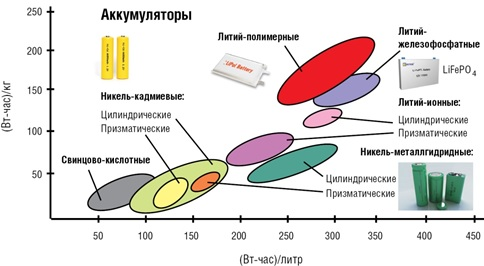
\includegraphics[width=.7\textwidth]{2164-1.jpg}
  \begin{quote}
    Abb. 1 -- Verteilung der verschiedenen Typen von elektrischen
    Akkumulatoren auf die Nischen mit Parametern spezifische Energie pro
    Einheit von Masse und Volumen
  \end{quote}
\end{center}

\begin{center}
  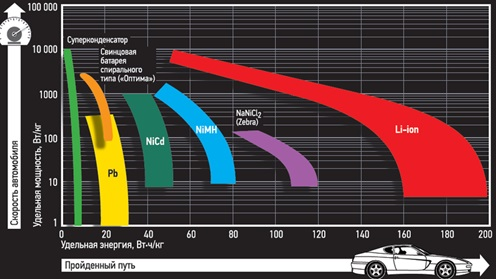
\includegraphics[width=.7\textwidth]{2164-2.jpg}
  \begin{quote}
    Abb. 2 -- Verteilung der verschiedenen Typen von elektrischen
    Traktionsbatterien (Akkumulatoren) elektrische Energie) in Nischen mit
    spezifischer Leistung und spezifischen Energieparametern (pro Einheit
    Massen)
  \end{quote}
\end{center}
Eine ähnliche Verteilung haben auch Baumaterialien in den Nischen. Zum
Beispiel, in Abb. 3 Die Abhängigkeit der Materialverteilung für die Gefäße von
der entsprechenden zu den parametrischen Nischen.
\begin{center}
  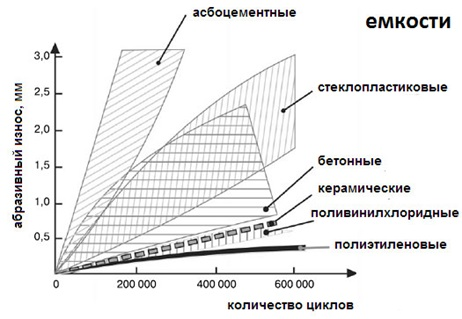
\includegraphics[width=.7\textwidth]{2164-3.jpg}
  \begin{quote}
    Abb. 3 -- Verteilung der verschiedenen Materialtypen für Gefäße in den
    Nischen mit Parametern zulässiger abrasiver Verschleiß und Anzahl der
    Lastzyklen
  \end{quote}
\end{center}
So kann man berücksichtigen, dass für Konstruktionen die Änderung eines
Materials eigentlich der Änderung von des Funktionsprinzips.

Im Gegensatz zur Funktion (GFP, EPF), die ein Spiegelbild der Ziele
(Bedürfnisse) der Gesellschaft ist, Funktionsprinzip bezieht sich auf das
natürliche Substrat als Mittel zur Ausführung einer Funktion.  Daher ist TS
als eine bestimmte Art von technischen Mitteln (ähnlich einem biologischen
Typ) ist es ratsam zu definieren, wie die Kombination (Einheit) des GPP und
das Funktionsprinzip der wichtigsten (zentralen) Subsysteme. Unter letzterem
wird ein solches Subsystem, EFF verstanden, das die Gruppe (Klasse) der TS
unterscheidet, vereint durch eine gemeinsame GFP, aus ähnlichen Systemen.
\emph{Zum Beispiel, für Systeme mit GUFs,„die Umsetzung von“.  Transport von
  Gütern auf der Wasseroberfläche“ wird das Haupt-(Zentral-)System ein
  Untersystem sein, sicherzustellen, dass das ESP„das Fahrzeug auf der
  Wasseroberfläche hält“, da die übrigen ESPs für fast alle Fahrzeuge, die
  Transportleistungen erbringen, typisch sind die Ladung}.

Eine Nischenbetrachtung der Handlungsprinzipien ist recht nützlich, erstens,
weil sie ein ziemlich vollständiges Bild der tatsächlichen Möglichkeiten
einiger oder anderer technologischer Effekte.  Zweitens erfordert die Arbeit
mit funktionalen parametrischen Nischen die folgende Unterscheidung
wesentliche Parameter, die die Möglichkeiten der Handlungsprinzipien
quantitativ charakterisieren, auf um Funktionen auszuführen. Drittens, wenn
eine erhebliche unerwünschte Wirkung verursacht wird.  (NE) ist eine
Veränderung eines quantitativen Indikators, der eine Nischengrenze definiert,
dann am wahrscheinlichsten, es ist notwendig, das Funktionsprinzip zu ändern
(d.h. Übergang zu einem neuen Typ von TS).

Quantitative Funktionsmerkmale sind ebenso wichtig wie qualitative Merkmale.
Wenn die Bedingungen für die Akzeptanz des TS für die Gesellschaft in Bezug
auf das Funktionieren verallgemeinert werden sollen, gegeben, Zum Beispiel
erhalten wir in [13], [15] und [22] die folgende Reihe von Bedingungen:
\begin{itemize}
\item die Hauptnutzfunktion (HPF) des TS sollte qualitativ (inhaltlich) und
  quantitativ den Anforderungen der Gesellschaft und/oder des technischen
  Umfelds entsprechen;
\item die funktionelle Stabilität muss gewährleistet sein (einschließlich
  Zuverlässigkeit und Dauerhaftigkeit und auf äußere Einflüsse);
\item der erforderliche Grad der Kontrollierbarkeit des
  Funktionierungsprozesses muss gewährleistet sein;
\item es sollte die Bequemlichkeit der menschlichen Interaktion mit dem
  Fahrzeug (einschließlich der Bequemlichkeit des Managements) gewährleistet
  sein, wenn eine solche Interaktion vorgesehen ist.
\end{itemize}

In Fällen, in denen eine Weiterentwicklung der zuvor geschaffenen und bereits
funktionierenden TS stattfindet, quantitative Merkmale des Funktionierens
sozusagen in funktionsfähigem Zustand festgelegt werden, und zwar bei
basierend auf einer Analyse der Bedürfnisse der Gesellschaft und des
technischen Umfelds. In Fällen, in denen TS erstellt wird zum ersten Mal
(Pionier-Entwicklung), ist es nützlich, die Notwendigkeit der Überwindung
\textbf{parametrischer Schwellenwerte}, die die Leistung des Systems
charakterisieren [13]. \textbf{Physikalische} parametrischer Schwellenwert
definiert die Bedingungen für einen nachhaltigen Systembetrieb.  \emph{Zum
  Beispiel, damit das Flugzeug selbstbewusst fliegen, sollte der maximale Wert
  der erzeugten Auftriebskraft 10-20\% betragen.  um das Gewicht des Flugzeugs
  zu überschreiten. Und jedes Überwasserschiff in voller Ladung muss einen
  Anteil Rümpfe, die nicht in Wasser eingetaucht sind (Oberflächenbrett), was
  die Überlebensfähigkeit des Schiffes unter verschiedenen Bedingungen
  gewährleistet von äußeren Einflüssen}. Die \textbf{funktionelle}
parametrische Schwelle bestimmt das Niveau von quantitative Parameter des
Funktionierens, bei denen die geschaffenen technischen Mittel bereits kann nur
als eine Demonstrationsfahrt angesehen werden. \emph{Zum Beispiel wird ein
  Flussdampfer ein echtes Fahrzeug, wenn er durch eine Tankstelle gegen Die
  Strömungen entsprechen mindestens der Entfernung zwischen den beiden
  Yachthäfen. Und ein klares Zeichen dafür, dass wurde das Flugzeug nach einem
  Blerio-Flug in die Reihe der einsatzfähigen Fahrzeuge aufgenommen.  über den
  Ärmelkanal}.

Eine der bedingungslosen natürlichen Bedingungen der Fahrzeugleistung ist die
Bereitstellung von ein \textbf{bestimmtes erforderliches Mindestmaß an
  Konsistenz der TS-Struktur}. In [14] gab es Es hat sich gezeigt, dass
strukturelle Kohärenz eine systemimmanente Eigenschaft ist.  Unkoordinierte
Systeme sind nicht praktikabel. Gleichzeitig wurde vorgeschlagen, dass der
Harmonisierungsprozess geteilt werden sollte TS in zwei Stufen: die erste
Stufe der Leistungssicherung -„\textbf{Schwellenwertvereinbarung}“, und
weitere„\textbf{Optimierungskoordination}“. Die Schwellenwerte werden
natürlich rechtzeitig angeglichen.  (gilt als erfüllt, wenn die
Betriebsfähigkeit des Fahrzeugs erreicht ist), und quantitative Bedingungen
des Schwellenwerts Abkommen haben die Form von Ungleichheiten (“nicht
weniger“,„nicht mehr“). Optimierungskoordination kann über den gesamten
Lebenszyklus der TS und die quantitativen Bedingungen der Optimierung
Konsonanzen haben die Form von Gleichungen (Gleichungen). Um solche
Gleichungen nicht zu überstrapazieren.  ein mehrstelliger Begriff wie
“Vereinbarung“, kann ein anfänglicher (Schwellen-)Vereinbarungsprozess
implementiert werden um den in der Evolutionsbiologie verwendeten Begriff
“\textbf{Konjugation}“ zu bezeichnen [23]. Am .  bei der Implementierung der
Schnittstelle ist die Struktur notwendigerweise auf die Funktion abgestimmt,
und auch die Interaktion der Strukturelemente untereinander qualitativ und
quantitativ.

Als Ergebnis der Konjugation ist die \textbf{Konformität von Struktur und
  Funktion} der TS gegeben, d.h.  ein ziemlich wichtiges absolutes Gesetz der
Konstruktion. Es sei angemerkt, dass in [17] dieses Gesetz...  wird als
“Eignung für Funktion und Struktur“ formuliert, mit Nachweis der Objektivität
wird diese Korrespondenz hervorgehoben. Diese Tatsache lässt sich dadurch
erklären, dass der Übergang von Funktion zu Struktur, wie bei jedem Übergang
vom Ziel zum Medium, ist ein Syntheseverfahren, das in ist prinzipiell nicht
eindeutig im Ergebnis. Ein eindeutiger Übergang von einer Funktion zu einer
Struktur ist nur möglich in trivialen (stereotypen) Fällen und ist bei der
Suche nach neuen Lösungen praktisch nicht anzutreffen. Das ist richtig.
Gleichzeitig ist der Übergang von der Struktur zur Funktion ein analytisches
Verfahren mit einer bestimmten Ergebnis: Was ist die Struktur, was ist die
Zusammensetzung und das Zusammenspiel der Elemente, und was sind die
Funktionen, die von dieser Struktur durchgeführt werden. Gleichzeitig werden
innerhalb der Grenzen der eindeutig festgelegten Korrespondenz von Struktur
und Funktion ist auch eine gültige These über die Korrespondenz von Funktion
und Struktur.

In jedem Fall gibt es eine wichtige Implikation dieses Gesetzes: \textbf{die
  Entsprechung zwischen Komplexität und Komplexität}.  Funktionen und
Strukturen. Eine der Manifestationen dieser Korrespondenz ist das formulierte
R.U.Ashby„das Prinzip der notwendigen Vielfalt“ - die Vielfalt des
Managementsystems sollte nicht weniger Vielfalt des Kontrollobjekts [16]. Nach
diesem Prinzip, mit zunehmender Komplexität des Kontrollobjekts, sollte auch
die Komplexität des Kontrollsystems zunehmen.

Auf der Grundlage der genannten Konsequenz lässt sich ein \textbf{Gesetz der
  Aufrechterhaltung der Komplexität} formulieren, das manifestiert sich
hauptsächlich im Prozess der TS-Entwicklung. In Übereinstimmung mit diesem
Gesetz, zur Vereinfachung die Struktur des Systems nicht willkürlich ist. Es
ist notwendig, entweder die Funktion des Systems zu vereinfachen (sein Volumen
zu reduzieren), indem einige Funktionen auf das Supersystem übertragen werden,
oder, unter Beibehaltung der Komplexität der Funktion, die Komplexität
innerhalb der Struktur auf andere Systemebenen zu übertragen (um die
Funktionen der einzelnen Systemebenen zu komplizieren).  Elemente -
“funktionell - perfekte Gerinnung“ oder übersetzen die Komplexität auf eine
Mikroebene, Erschwerung der verwendeten Bewegungsform der Materie -„Änderung
des Funktionsprinzips des Teilsystems“).

\begin{emph}
  Durch die Wirkung dieses Gesetzes wird das in der TRIZ bekannte Phänomen,
  wie„die Welle der Vollkommenheit“. In der Anfangsphase dieser Welle wurde
  aufgrund der unterschiedlichen Funktionsweise der in Raum und Zeit, in
  Übereinstimmung mit dem Akt des Exzellenzgesetzes gibt es eine entsprechende
  Komplikation der Systemstruktur. Diese Komplikation führt zu Reduzierung der
  Zuverlässigkeit des Systembetriebs (NE), der ab einem bestimmten Moment
  einsetzt Vereinfachung der Struktur. Formen zur Erreichung der
  erforderlichen Vereinfachung (Übergang zu einem Supersystem, Übergang zum
  zur„idealen“ Substanz usw.) [24] entspricht durchaus dem Gesetz der
  Komplexitätserhaltung.  [13].
\end{emph}

Bei dem Prozess der Verknüpfung von Elementen in der Struktur des TS ist es
auch notwendig, ein \textbf{Minimum von das für die Funktionsfähigkeit
  erforderliche Maß an Systemsteuerbarkeit}. Wie bereits erwähnt,
Beispielsweise können Sie in [16] nur ein dynamisches System steuern,
d. h. ein System, das rechtzeitig, um verschiedene Zustände in einem durch das
inhärente System definierten Bereich zu akzeptieren mit Freiheitsgraden. Doch
nicht alle dynamischen Systeme erfordern ein Management. Kontrolle wie...  die
gezielte Einwirkung auf das System durch das jeweilige Teilsystem erforderlich
ist, wenn die folgenden Bedingungen erfüllt sind:
\begin{itemize}
\item das System in einigen seiner Staaten dynamisch ist;
\item Es besteht die Notwendigkeit, das System in einen bestimmten Zustand aus
  den Reihen möglich (und/oder es in diesem Zustand zu halten);
\item es nicht möglich ist, das System durch den Basisprozess in den
  erforderlichen Zustand zu bringen des Funktionierens.
\end{itemize}
\begin{emph}  
  Zum Beispiel, wenn ein Gegenstand auf Stoßdämpfern montiert ist, um zu
  verhindern der Ausbreitung des Vibrationsflusses, dann erlangt er viele
  Freiheitsgrade und wird...  dynamisch. In den meisten Fällen ist die
  Aufrechterhaltung eines bestimmten Zustandes von der ursprünglichen Viele
  mögliche Staaten sind einfach nicht erforderlich: all diese werden als
  akzeptabel angesehen. Es gibt eine Reihe von wo eine niederfrequente
  (“weiche“) Abschreibung angewendet wird, ist es notwendig den Umfang der
  Bewegung des Objekts in einigen Einsatzsituationen begrenzen. In diesem In
  den meisten Fällen werden zusätzlich zu den Niederfrequenz-Stoßdämpfern auch
  Hochfrequenz-Stoßdämpfer eingesetzt.  (“harte“) Stoßdämpfer, die nach
  Überschreiten eines bestimmten Abschreibungsniveaus in Betrieb genommen
  werden.  den Wert der Bewegungen des Objekts (aufgrund der Tatsache, dass
  das Objekt einfach mit„harten“ Gegenständen in Berührung kommt)
  Stoßdämpfer). Es sind keine besonderen Kontrollmaßnahmen
  erforderlich. Allerdings .  Es gibt Betriebsbedingungen, unter denen eine
  Bewegung des Objekts nicht zulässig ist.  In diesem Fall besteht die
  Notwendigkeit einer gezielten Abschaltung der Abschreibung, die durchgeführt
  wird für durch die Einführung eines geeigneten Steuerungssubsystems
  (z.B. durch die Erweiterung der von starren Verankerungen).
\end{emph}

Es ist zu beachten, dass die Bedürfnisse der Gesellschaft dem Bedürfnis
entsprechen, das Objekt an die eine Bedingung und/oder Beibehaltung dieser
Bedingung. Gezielte Kontrolle durch ein geeignetes dediziertes Subsystem dafür
ist nur ein Mittel (und am häufigsten gezwungen). Um die Effizienz des
Fahrzeugs zu gewährleisten, ist es daher notwendig, in erster Linie Folgendes
zuzuweisen Es ist die Art von Kontrollaktionen, ohne die das System wirklich
nicht funktionieren kann.

Da die meisten TS durch einen Prozess gekennzeichnet ist, der ihr
Funktionieren gewährleistet, ist es notwendig Notwendige Kontrollmaßnahmen in
solchen Fällen sind die Anlaufvorgänge und Betriebsunterbrechungen. Andere
notwendige Kontrollmaßnahmen werden festgelegt die Besonderheiten der
Funktionsweise und die Funktionsprinzipien der Teilsysteme. \emph{Zum Beispiel
  für eine Dampfturbine.  Das erforderliche Mindestmaß an Regelbarkeit kann
  durch das Teilsystem gewährleistet werden, die den Dampffluss gewährleistet
  und diesen Fluss stoppt. Wenn die Turbine funktioniert sieht eine
  Geschwindigkeitsänderung und/oder Stabilisierung vor, um dann Es wird
  notwendig sein, ein geeignetes Steuerungssubsystem hinzuzufügen.  Dasselbe
  Muster ist bei der Dampfmaschine zu beobachten. Da jedoch sein
  Funktionsprinzip nimmt zyklische Bewegung des Kolbens mit entsprechender
  Änderung der Arbeitsströme an und Abdampf, muss auch in der Dampfmaschine
  ein Teilsystem vorhanden sein.  Steuerung der vorgegebenen Flüsse (synchron
  mit der Kolbenbewegung)}.

In einigen Fällen besondere Dynamik einiger Parameter des Systems, das eine
Zielsteuerung erfordert, ist auf den Einfluss des Umfelds zurückzuführen, in
dem die TS tätig ist.  \emph{Ein Überwasserschiff kann zum Beispiel um sich
  auf allen drei Achsen zu bewegen und zu drehen. Allerdings sind sowohl
  vertikale Bewegungen als auch Rotationswinkel relativ zu den horizontalen
  Achsen (Rollen und Trimmen) werden durch die werden durch die Auswirkungen
  der aquatischen Umwelt begrenzt und durch die Auswirkungen der Schwerkraft
  der Erde begrenzt. Und die Drehungen und Wendungen Auf der vertikalen Achse
  (Kurswinkel) gibt es keine natürlichen Einschränkungen. Daher gilt auf
  Schiffen müssen Sie ein Kurswinkelsteuerungs-Subsystem installieren}.

In der Regel sollte die Synthese des Regelungssubsystems mit der Bestimmung
der Art der Auswirkungen auf die ein dynamisches Objekt oder einen Teil davon,
wodurch Sie das Objekt in den gewünschten Zustand bringen können. Dann unter
diese Art des Aufpralls auf das Objekt wird unter Berücksichtigung des
Funktionsprinzips des Steuerungssubsystems ausgewählt die im System und/oder
in seiner Umgebung verfügbaren Ressourcen.  \emph{Noch einmal, zum Beispiel
  die Über-Wasser ein Schiff, wir bekommen das, um das Schiff auf der
  Kurskurve um die vertikale Achse auf dem Schiff zu drehen, ist es notwendig
  mit einem horizontal wirkenden Moment zu handeln. Für ein fahrendes Schiff.
  Eine der einfachsten Möglichkeiten, einen solchen Moment zu schaffen, ist
  die Schaffung einer der hydrodynamischen Kraft in einem der Enden des
  Rumpfes (es ist effizienter, eine solche Leistung im Heck). Um die
  erforderliche hydrodynamische Kraft zu erzeugen, wurde ein Flügel (Platte)
  in das Wasser gestellt, die sich relativ zur vertikalen Achse drehen könnte,
  wodurch der erforderliche Anstellwinkel.., bzw. die erforderliche Kraft- und
  Drehmomentmenge. Und diesen Flügel (Ruder) in der Zusammensetzung von das
  Steuersystem muss mindestens den Antrieb einschalten, der seinerseits von
  einem menschlichen Wesen kontrolliert zu werden}.

Wenn sich der Objektzustand aufgrund bestimmter Transformationen irgendeines
Flusses ändert, dann ist für Die Bewältigung des Wandels bei diesem Wandel ist
eine der strukturellen Verbindungen, die der Strom sollte den notwendigen
Einfluss auf den Strom und die strukturelle Verbindung selbst in seine eigene
die Warteschlange muss empfänglich sein für die entsprechende
Zielsteuerungsaktion (d.h.  soll variabel sein).

In [17] werden als Konstruktionsgesetze die \textbf{Symmetriegesetze der
  technischen Objekte} erwähnt, in nach der ein technisches Objekt, das eine
bestimmte signifikante Auswirkung hat Umwelt in Form von Stoff-, Energie- oder
Informationsflüssen eine bestimmte Art von Symmetrie aufweist, aufgrund der
Kombination und Art dieser Ströme. Tatsächlich sind die meisten Transporte
Mittel zum Beispiel symmetrisch in Bezug auf die vertikale Ebene sind, die
entlang der zur Fahrtrichtung dieser Fahrzeuge. Dies ist auf die Schwerkraft
der Erde zurückzuführen, und das Fehlen einer solchen Schichtung der
Auswirkungen in horizontaler Flugzeuge. Dieses Phänomen sollte jedoch
\textbf{nicht als Gesetz, sondern als natürliche Tendenz} betrachtet werden,
weil es bekannte Ausnahmen von der Symmetrie gibt im Fall von Der symmetrische
und homogene Einfluss des Mediums ermöglicht eine Optimierung der TK (siehe
z.B. [25]). Thema Nicht weniger verdienen die in [17] aufgeführten Regeln
Aufmerksamkeit, Untersuchung und Einbeziehung in die Umlaufbahn der TRIZ.

Jede Symmetrie ist in der Tat eine Einschränkung der Vielfalt. Das ist im
Falle einer Gleichförmigkeit der Einflüsse der Fall.  Umfeld oder Funktion,
wird auch in der Struktur eine entsprechende Reduktion der Vielfalt
realisiert. Mit anderen Worten.  Hier geht es darum, das Gesetz der
Übereinstimmung zwischen Struktur und Funktion aufzuzeigen.

\section*{Quellen}
\begin{description}
\item[1.] G.S. Altschuller. Kreativität als exakte Wissenschaft. Moskau, 1979.
\item[2.] V.M. Petrov. Gesetze der Entwicklung TS. Bericht auf dem Seminar der
  TRIZ-Entwickler (Petrosawodsk 1982). Leningrad, 1982.
\item[3.] V.M. Petrov. Gesetzmäßigkeiten der Entwicklung technischer Systeme.
  In: Methodik und Methoden technischer Systeme.  der Kreativität. Thesen von
  Berichten und Botschaften an die wissenschaftlich-praktische Konferenz.
  Nowosibirsk, 1984. S. 52-54.
\item[4.] B.I. Goldovsky. Gesetzmäßigkeiten der Konstruktion und Entwicklung
  technischer Systeme (1981-1983).
  \url{http://triz-summit.ru/ru/205253/203840/Gold/303251/} 
\item[5.] B.I. Goldovsky. Probleme der Modellierung der Entwicklung
  technischer Systeme (auf Russisch).  Entwicklung regionaler
  wissenschaftlich-technischer Systeme.  praktische Konferenz„Probleme der
  Entwicklung der wissenschaftlichen und technischen Kreativität der
  ITR“. Thesen reports - Gorki, 1983.
\item[6.] B.I. Goldovsky. Noch einmal zum Platz der TRIZ (2013).
  \url{http://www.metodolog.ru/node/1593}. 
\item[7.] V.M. Petrov. Die Gesetze der Systementwicklung. Monographie. Tel
  Aviv, 2013.
 \item[8.] A.L. Lubomirski, S.S. Litvin. Gesetze der Entwicklung technischer
   Systeme. GEN3-Partner, 2003.
   \url{http://www.metodolog.ru/00767/00767.html}. 
\item[9.] L.S. Salamon. Über einige Faktoren, die die Wahrnehmung eines neuen
  Wortes in der Wissenschaft bestimmen (auf Russisch). In: Wissenschaftlich.
  Entdeckung und ihre Wahrnehmung. Moskau, 1971, S. 113.
\item[10.] N.A. Shpakovsky. Gesetze der Systementwicklung und Linien ihrer
  Entwicklung. In: Sammlung von Berichten der IX internationalen Konferenz
 „TRIZ. Praxis der Anwendung und Entwicklung von methodischen Werkzeugen“.
  Moskau, 10.-11. November 2017. Band 2, S. 177-190.
  \url{http://trizofication.ru/conference2017}. 
\item[11.] B.I. Goldovsky. Über Widersprüche in technischen Systemen. Teil 2.
  Nischnij Nowgorod, 1999. Hinterlegt im ChOUNB 28.02.2000 Nr. 2547.
  \url{http://www.metodolog.ru/00001/00001.html}.
\item[12.] B.I. Goldovsky. Einige Reflexionen über das Wesen der TRIZ. (2017)
  \url{http://triz-summit.ru/205253/203840/gold/303614}
\item[13.] B.I. Goldovsky, M.I. Vainerman. Rationale Kreativität. Moskau,
  1990.
\item[14.] B.I. Goldovsky. über das Gesetz der„Harmonisierung technischer
  Systeme“. (2013) \url{http://www.metodolog.ru/node/1632}
\item[15.] B.I. Goldovskiy. Über Spezialisierung, Universalisierung und
  Hybridisierung. Sammlung von Berichten der VIII internationalen Konferenz
 „TRIZ: Praxis der Anwendung und Probleme der Entwicklung“. Moskau
  11.-12. November 2016. S. 213-228
\item[16.] B.I. Goldovsky. Über Dynamik und Handhabbarkeit technischer Systeme
  (2017) \url{http://www.metodolog.ru/node/2041};
  \url{http://triz-summit.ru/205253/203840/Gold/303482/}
\item[17.] A.I. Polovinkin. Grundlagen der Ingenieurskreativität: Lehrbuch,
  Handbuch für Studenten höherer Bildungseinrichtungen. Moskau, 1988.
\item[18.] B.I. Goldovsky. Ist es möglich, Perfektion zu messen? (Anmerkungen
  zum zentralen Muster der TRIZ) (2012).
  \url{http://www.metodolog.ru/node/1484}.
\item[19.] R. Koller. Konstruktionsmethode für den Maschinen-, Geräte- und
  Apparatebau. Berlin, 1976.  Russ. Übersetung unter
  \url{http://www.metodolog.ru/00348/00348.html}. 
\item[20.] Yu. Khotimlyansky. Energieanalyse technischer Systeme. Baku, 1974. 
\item[21.] B.I. Goldovsky et al. Eine umfassende Methode, um neue technische
  Lösungen zu finden. In 3 Teilen. Gorki, 1979, 1980.
\item[22.] C.M. Christensen. The Innovator's Dilemma. Warum etablierte
  Unternehmen den Wettbewerb um bahnbrechende Innovationen verlieren. München,
  2011.  (Englisches Original 1997)
\item[23.] Yu.M. Tschaikowsky. Aktive vernetzte Welt. Erfahrung mit der
  Theorie der Evolution des Lebens. Moskau, 2008.
\item[24.] I.M. Kondrakow. Die Welt kennen lernen. Lehrbuch. St. Petersburg,
  2015.
\item[25.] B.I. Goldovsky.  Originale Flugzeuge von Bert Rutan (2016).
  \url{http://triz-summit.ru/ru/205253/203840/Gold/302917/}. 
\end{description}

\end{document}
